\section{Results and Analysis}\label{sec:results}

The three contributions concern regional allocation, last-layer expressivity and spectral
weighting. We first compare uncertainty with realised error, then examine the features and
curvature that determine these quantities.

\subsection{Regional Allocation, Scale Sensitivity, and Predictive Centres}\label{sec:ceiling}

The comparisons retain the training-weighted homoscedastic likelihood, original
reference regions and trained-network admission decisions. Burgers--MLP supplies
eight unfiltered seeds; the other nonlinear families are smaller selected samples.

\emph{Regional allocation and scale sensitivity.}
Every admitted nonlinear run has a baseline allocation deficit (Table~\ref{tab:ceiling}).

\begin{table}[t]
\centering\small


\begin{tabular}{@{}lcccc@{}}
\toprule
configuration & admitted & $\Rrms$ & $\Rtar$ & $\ratiogap$ \\
\midrule
Burgers, MLP & $8/8$ & $6.37\pm0.38$ & $130.6\pm82.4$ & $20.5\pm13.1$ \\
Burgers, Fourier & $3/8$ & $[3.857,3.959]$ & $[15.77,116.5]$ & $[4.09,29.55]$ \\
Allen--Cahn, MLP & $3/5$ & $[6.871,7.731]$ & $[21.58,33.58]$ & $[2.958,4.888]$ \\
Allen--Cahn, Fourier & $3/4$ & $[5.818,5.93]$ & $[12.64,17.37]$ & $[2.165,2.986]$ \\
\midrule
configuration & $\meanZ_{\mathcal S}$ & $\meanZ_{\mathcal B}$
 & $\mathrm{cov}@68_{\mathcal S}$ & $\mathrm{cov}@68_{\mathcal B}$ \\
\midrule
Burgers, MLP & $0.319\pm0.275$ & $0.012\pm0.003$ & $0.923\pm0.083$ & $1.000\pm0.000$ \\
Burgers, Fourier & $[0.3996,0.724]$ & $[0.02456,0.1248]$ & $[0.8227,0.8912]$ & $[0.9997,1]$ \\
Allen--Cahn, MLP & $[0.1845,0.3296]$ & $[0.02925,0.03078]$ & $[0.9708,1]$ & $1$ \\
Allen--Cahn, Fourier & $[0.2533,0.2893]$ & $[0.02237,0.0284]$ & $[0.9958,1]$ & $1$ \\
\bottomrule
\end{tabular}
\caption{Unit-noise, plug-in-precision baseline with trained centres. Burgers--MLP entries
are mean $\pm$ population standard deviation over eight admitted seeds; other entries are
observed ranges over three admitted runs. Counts are admitted/attempted.
Ranges are descriptive, not confidence intervals. Calibration benchmarks are
$\meanZ\approx0.8$ and one-standard-deviation coverage $\approx0.68$.}
\label{tab:ceiling}\label{tab:absolute}
\end{table}

For canonical Burgers--MLP seed $2$, $(\Rrms,\Rtar,\ratiogap)=(6.47,118.58,18.3)$.
Across Burgers--MLP seeds, $\Rrms$ varies by $6\%$ (coefficient of variation), over
$[6.00,7.25]$, whereas $\Rtar\in[10.0,238.2]$. All eight attempted seeds pass admission,
so this family's deficit is not an admission-selection effect. Small bulk-error denominators
amplify target variation; the bulk is also strongly over-dispersed at this baseline.

\begin{table}[t]
\centering\small


\begin{tabular}{@{}lccccc@{}}
\toprule
window & $\Rrms$ & $\ratiogap$ & $\meanZ_{\mathcal S}$ & $\mathrm{cov}@68$ & $\mathrm{cov}@95$ \\
\midrule
$t<1/\pi$ & $2.65\pm0.23$ & $16.9\pm14.5$ & $0.10\pm0.07$ & $0.99\pm0.01$ & $1.00\pm0.00$ \\
$t\ge1/\pi$ & $10.75\pm0.71$ & $20.6\pm13.1$ & $0.81\pm0.81$ & $0.76\pm0.27$ & $0.87\pm0.17$ \\
\bottomrule
\end{tabular}
\caption{Burgers--MLP baseline split at $t=1/\pi$, with trained centres; mean $\pm$
population standard deviation over eight seeds. Coverage and $\meanZ$ concern the sharp
region. Pre-formation points constitute $69\%$ of the global sharp mask.}
\label{tab:temporal}
\end{table}

The global mask mixes pre- and post-formation behaviour (Table~\ref{tab:temporal}).
The mean gap exceeds one in both windows, so early points are not its sole source.
Post-formation sharp coverage varies over $[0.37,1.00]$ and $\meanZ_{\mathcal S}$ over
$[0.02,2.43]$, while $\Rrms\in[9.93,12.37]$: similar contrasts can accompany very
different calibration. Allen--Cahn has no sharp points before $t\approx0.4$ under the
same global-percentile rule.

The baseline contrast also changes by at most $1.1\%$ between the two finest evaluation subsamples
(Appendix~\ref{app:grid}); Gaussian and Student-$t$ distributions with matched covariance
have identical RMS and mean-width contrasts.

The scale sweep covers all $17$ admitted nonlinear checkpoints with residual weights
and reference regions fixed, using trained and zero-mean-prior affine centres. Burgers also uses
the global masks intersected with $t\ge1/\pi$. The unit-noise
sweep contains $19$ prior multipliers from $10^{-7}$ to $10^2$ and matched points for the
conditional noise MLE and finite-grid evidence selections. A centre change preserves
$\Rrms$ at fixed $\gamma$, but changes the target and calibration diagnostics.

Five trained-centre Burgers--MLP seeds cross $\ratiogap=1$ in the observed brackets
(Figure~\ref{fig:n1-scales}). Saved modal sums refine the crossings to a range from
$2.05\times10^{-5}$ (seed $5$) to $0.736$ (seed $4$), more than four orders of
magnitude apart in effective precision (Table~\ref{tab:r3-roots}). The original sampled
brackets are listed in Appendix~\ref{app:n1}. Seeds $1$--$3$ remain above one, with minimum
sampled gaps $1.84$, $2.59$ and $1.99$ (Appendix~\ref{app:n1}). Seeds vary in both
error target and weak-precision geometry: baseline uncertainty contrast varies by $6\%$,
while each seed's largest sampled contrast ranges from $45.83$ to $517.34$.
The QR-complement RMS ratios span $[42.71,509.9]$ (Table~\ref{tab:r2-limits}).
This complement is orthogonal to the retained $N$-column QR factor for $J^\top$
(Appendix~\ref{app:r2:numerics}); its ratios identify the whole-kernel limit only
under the rank condition in Section~\ref{sec:theory}.

\begin{figure}[t]
\centering
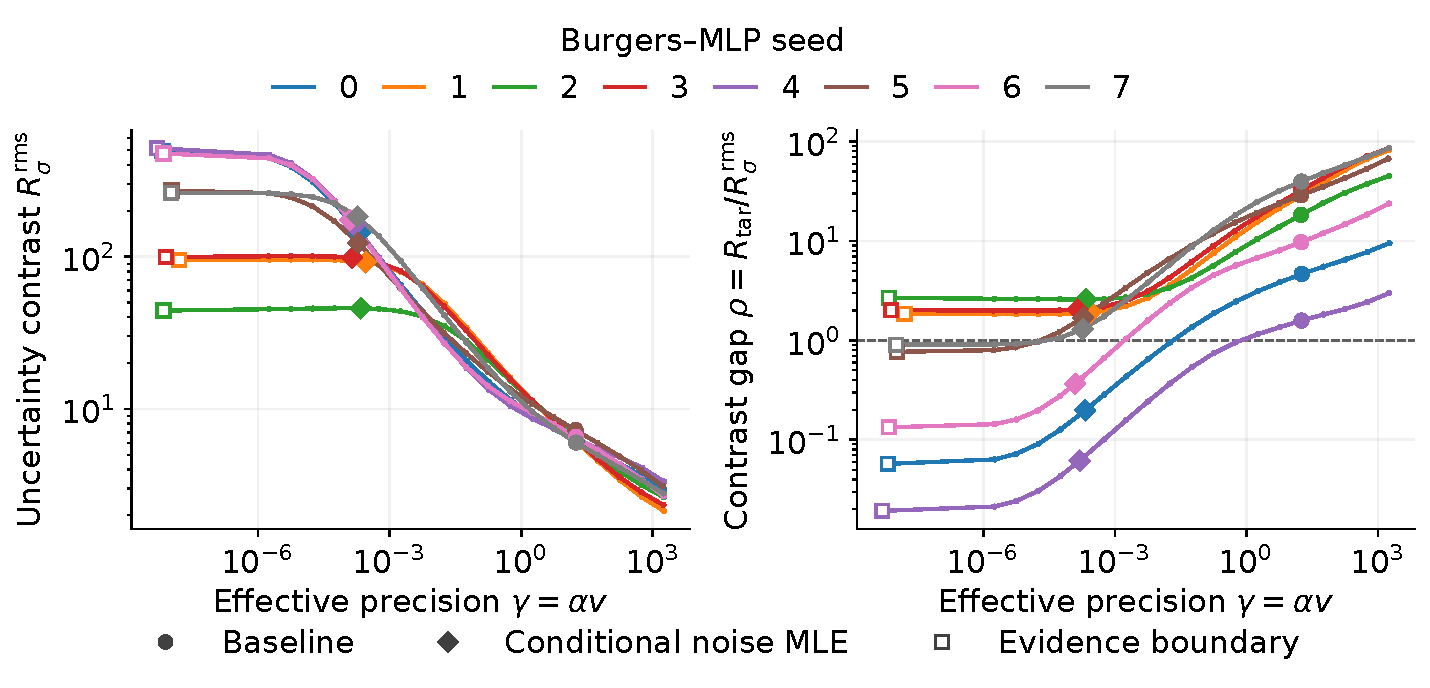
\includegraphics[width=0.96\textwidth]{figures/round2_contrast_and_gap.pdf}
\caption{Uncertainty contrast (left) and gap $\ratiogap=\Rtar/\Rrms$ (right) for eight
Burgers--MLP seeds with trained predictions fixed. Curves join $19$ unit-noise prior
settings and exact matched MLE/original-evidence points. Circles mark the baseline
$(\alpha_0,1)$, diamonds the conditional noise MLE $(\alpha_0,\widehat v)$, and open
squares the best original-grid evidence setting at the lower noise boundary. Selected
settings share contrasts with their unit-noise aliases, but not absolute widths. The
dashed line marks equal RMS contrasts, not calibration. Appendix~\ref{app:r2} summarises
other families, affine centres and extended-grid diagnostics; Appendix~\ref{oa:empirical} gives
their full curves.}
\label{fig:n1-scales}
\end{figure}

\emph{Training-based scale choices.}
The conditional MLE $\widehat v=\|r(\theta)\|^2/N$ fixes the trained parameter.
Fitted-residual reuse can underestimate variance; this plug-in residual scale is
not an unbiased discrepancy estimate. No classical degrees-of-freedom correction
is assigned here (Appendix~\ref{oa:numerics}). With trained centres it reverses
the allocation deficit in seeds $0$, $4$ and $6$; the other five have
$\ratiogap\in[1.30,2.59]$. Nevertheless, all eight seeds under-cover both regions:
one-standard-deviation coverage is $0.198$--$0.416$ in bulk and $0.018$--$0.5315$ in sharp;
at $1.96$ standard deviations it is $0.412$--$0.721$ and $0.051$--$0.698$.

On both zero-mean-prior evidence grids, $14/17$ best tested pairs lie at the lowest allowed noise
variance; extending the range does not resolve those boundary selections.
The three Allen--Cahn Fourier candidates are interior, whereas singular-value
perturbations substantially change Allen--Cahn MLP selections. These are finite-grid
candidates rather than reliably identified scales. Appendix~\ref{app:r2:evidence}
records the projected-data mechanism, extension and numerical sensitivity.

\emph{Predictive centres and linearisation.}
At the baseline, the zero-mean-prior affine centre increases full-grid error RMS in $14/17$ checkpoints
(Table~\ref{tab:r2-centres}). For Burgers--MLP, mean $\Rtar$ falls from $130.6$ to $13.13$
and mean $\ratiogap$ from $20.47$ to $2.09$, but mean sharp error RMS rises from $0.1138$
to $0.2448$ and bulk error RMS from $0.000805$ to $0.01821$; sharp error worsens in seven
of eight seeds. Thus a reduced target can accompany worse prediction.

The displacement separates as $\delta_\gamma=\delta_{L,\gamma}+\delta_{P,\gamma}$,
where the likelihood term is the shift under the $\theta$-centred prior and
$\delta_{P,\gamma}=-\gamma(F+\gamma I)^{-1}\theta$ is prior shrinkage. Its QR-complement
term is $-\theta_c$ at every scale, where $\theta_c$ is the parameter projection
onto that complement. At the baseline, total displacement is
$99.78$--$99.96\%$ of $\|\theta\|$, whereas the likelihood term is at most
$0.0155\%$. Prediction-level bounds establish prior-only worsening in all $14$
affected runs (Appendix~\ref{app:r3:centres}); parameter norms alone would not
establish that attribution.

For the $\theta$-centred prediction, the pointwise baseline shift bound ranges from
$0.00749$ to $0.0908$ standard deviations. Bounds establish $\rho>1$ in $16/17$;
direct evaluation gives $\rho>1$ in all $17$, resolving Burgers--MLP seed $4$ with gap $1.582$.
Both regions over-cover at one standard deviation. At the conditional-MLE
scales, $\rho^\theta\in[2.18,10.01]$. The affine mean improves full-grid RMS error
in $15/17$ runs (Table~\ref{tab:r2-centres}), with median error ratio $0.7953$.
At one standard deviation, all $17$ bulk regions over-cover and $12/17$ sharp regions
under-cover. Thus prediction can improve without
regional calibration. The residual variance is not re-estimated after shifting.

At the baseline, nonlinear evaluation $u_{\theta+\delta_{L,\gamma}}$ also retains
$\rho>1$ in all $17$, with regional RMS affine remainder below $6.4\times10^{-4}$
of RMS $\sigma$. At the MLE, however, the bulk remainder is $2.495$--$386.16$ times
RMS $\sigma$, despite $\|\delta_L\|/\|\theta\|\in[0.00782,0.03867]$.
Full-grid error worsens in $11/17$ and bulk error in all $17$.
Observed nonlinear gaps below one reflect bulk deterioration, not repaired allocation.
These are forward diagnostics with covariance frozen at $\theta$.

\emph{Oracle: contrast agreement and coverage.}
A descriptive oracle rescales each saved covariance to target $68\%$ bulk coverage using the
higher empirical quantile of $|e|/\sigma$, separately for each centre and time subset.
It uses reference errors and is not a practical tuning rule. For the five trained-centre
bracketing seeds, the closest saved points have $\ratiogap\in[0.954,1.032]$, yet sharp
coverage is $0.343$--$0.652$ at one standard deviation and $0.692$--$0.864$ at $1.96$.
For zero-mean-prior affine post-formation predictions, the closest points across all eight seeds have
$\ratiogap\in[0.933,1.193]$ and sharp one-standard-deviation coverage $0.009$--$0.347$.
At the five refined trained-centre roots, direct sharp coverage is
$0.30325$--$0.55725$ at one standard deviation and $0.67725$--$0.852$ at $1.96$
(Table~\ref{tab:r3-roots}). All values lie within the positive-modal envelopes,
whose upper bounds are at most $0.563$ and $0.862$, respectively
(Appendix~\ref{app:r3:root-envelope}). Contrast agreement therefore does not
restore sharp coverage under this bulk calibration.

At these five trained-centre roots, the $\theta$-centred affine prediction has
full-grid error RMS $0.493$--$0.973$ times that of the trained prediction and
$\rho^\theta\in[1.13,7.58]$; these precisions do not match its own error contrast.
After its own bulk-$68\%$ calibration, sharp one-standard-deviation coverage is
$0.1165$--$0.424$.

For $Z_j=e_j/\sigma_j$, define the variance-weighted regional second moment
\[
 M_r=\frac{\sum_{j\in r}\sigma_j^2Z_j^2}{\sum_{j\in r}\sigma_j^2}
     =\frac{\langle e^2\rangle_r}{\langle\sigma^2\rangle_r},\qquad
 \rho^2=M_{\mathcal S}/M_{\mathcal B}.
\]
Thus $\rho=1$ equates weighted second moments, leaving ordinary coverage quantiles
undetermined. At the five nearest saved oracle settings, using bulk-calibrated widths,
sharp median $|Z|$ ranges
over $[0.725,1.273]$, compared with $[0.655,0.701]$ in bulk; sharp $99$th percentiles
are $3.60$--$8.70$, versus $3.05$--$4.66$ in bulk. Sharp signed means include
$-1.96$ (seed $5$) and $0.85$ (seed $7$). The top $1\%$ of sharp points carry $15.3$--$23.8\%$ of error
energy, and width--absolute-error Spearman rank correlations are $0.693$--$0.936$.
Larger sharp medians show that the difference extends beyond extreme tails;
regional sign bias and substantial width--error ordering coexist with undercoverage.

An RMS deficit can coexist with overcoverage: seed $1$ has closest gap $1.836$
and sharp one-standard-deviation coverage $0.8605$; seed $3$ has gap $1.992$
and coverage $0.725$ (Tables~\ref{tab:r2-oracle} and~\ref{tab:r4-oracles}).

Sharp calibration using its higher empirical $0.68$ quantile gives sharp
$1.96$-standard-deviation coverage $0.8345$--$0.95775$ for Burgers--MLP, below
$0.95$ in $7/8$ runs. Other families and time subsets include overcoverage
(Table~\ref{tab:r4-oracles}): matching one quantile need not match another.
This output rescaling preserves within-region width patterns and does not test
a residual-informed likelihood that changes $J^\top D^{-1}J$.

In the sampled band $0.9\le\rho\le1.1$, Burgers--MLP seed $7$ has seven
settings with sharp one-standard-deviation coverage $0.44725$--$0.986$ after
bulk calibration: $\rho=0.925$ gives $0.756$, while $\rho=1.064$ gives $0.44725$.
These include undercoverage and overcoverage, without a continuous-band claim
(Appendix~\ref{app:r4-oracles}).

\emph{Ensemble comparison.}
An ensemble \citep{lakshminarayanan2017ensembles} of the eight Burgers--MLP runs, with
spread computed at divisor $K=8$, has $\Rrms=136.5$, its own mean-prediction target
$\Rtar=158.2$ and $\ratiogap=1.16$. Sharp $\meanZ=0.64$ and coverage is $0.876/0.993$
at $68/95\%$, while bulk $\meanZ=0.45$. It nearly matches allocation but does not restore
absolute calibration. The ordering against individual Gaussians depends on their scale:
at the conditional MLE three trained-centre gaps are below one and five lie in
$[1.30,2.59]$, each relative to its own predictor's error. Omitting one ensemble member
gives gaps $1.055$--$1.351$, sharp $68\%$ coverage $0.4935$--$0.9075$ and $95\%$ coverage
$0.9720$--$0.9995$. Omitting seed~$5$ gives the largest gap and lowest $68\%$ coverage;
its sharp error has correlation $-0.7517$ with the other seven's mean error. These ranges
measure membership sensitivity, not confidence intervals: each omission changes the
predictor, target and spread.

